% třída dokumentu
\documentclass[10pt]{article}

% použité balíčky
\usepackage{graphicx}
\usepackage{subcaption}
\usepackage{booktabs}
\usepackage{geometry}
\geometry{height=10in,a4paper,hmargin={3cm,0.8in}}
\usepackage[utf8]{inputenc}
\usepackage[T1]{fontenc}
\usepackage{amsmath}
\usepackage{hyperref}
\usepackage{multirow}
\usepackage{lmodern}
\usepackage{amsfonts}
\usepackage[czech]{babel}
\begin{document}
\title{SKE - Zápočtová úloha}
\author{Miroslav Kubů}

\maketitle
\setlength{\footskip}{28pt}

\section{Úvod}
V této práci se zabýváme modelováním času dožití $T$ na základě dat o 137 pozorovaných pacientech. Data byla sbírána po období 1000 dnů, poté byl sběr dat ukončen. Z tohoto důvodu máme v datové množině též 9 cenzurovaných pozorování. Rozdělení četností doby dožití pacientů $t$ udávadané ve dnech zobrazujeme na obrázku \ref{fig:histo}. Z něj je tak patrné, že vysoké množství pacientů zemřelo již krátce po začátku měření. Průměrný věk dožití činí 121.6 dnů, medián nicméně činí pouze 80 dnů. Veliký rozdíl mezi průměrem a mediánem je způsoben právě skupinou 9 cenzurovaných pozorování, u nichž je uvedena doba dožití 1000 dnů, což významně ovlivňuje výpočet průměru.
\begin{figure}[htb!]
\centering
    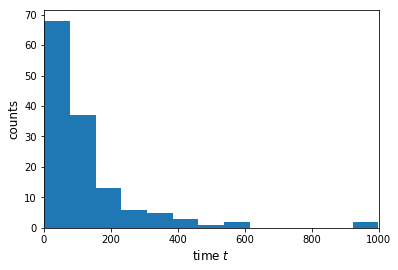
\includegraphics[width=.6\textwidth]{Images/hist.png}
  \caption{Vykreslení četností času dožití.}\label{fig:histo} 
    \end{figure}
V rámci datové množiny máme ke každému pozorování k dispozici 6 parametrů popisujících pacientovo Karnofsky skóre, typ rakovinových buněk, věk pacienta a typ léčby. V rámci této práce se poté snažíme pozorovat rozdíly v časech dožití pro různé podskupiny pacientů. Jednotlivé modely vyhodnocujeme na základě spolehlivostní funkce $R(t)$, jež pro náhodnou veličinu $T \in \mathbb{R}^+$ s distribuční funkcí $F(t)$ definujeme v čase $t$ jako 
\begin{equation}\label{spol}
R(t)=\textrm{P}(T>t)=1-F(t).
\end{equation}
Spolehlivostní funkce tedy odpovídá pravděpodobnosti přežití do času $t$. Další pozorovanou funkcí je intenzita poruch definovaná jako
\begin{equation}\label{poruch}
r(t)=\frac{f(t)}{R(t)},
\end{equation}
kde $R(t)$ je spolehlivostní funkce a $f(t)$ hustota pravděpobnosti pro náhodnou veličinu $T$. Numericky poté porovnáváme časy dožití pro jednotlivé skupiny skrze střední dobu života $ \textrm{E}[T]$. Kromě střední doby života pozorujeme též mediánovou dobu života.

\section{Použité modely}

V rámci analýzy času přežití $T$ pro různé podskupiny pacientů zkoumáme vliv faktorů jako Karnofsky score, typu buněk, věku pacientů a způsobu léčby na čas přežití. K tomu používáme neparametrické i parametrické modely.

Neparametricky lze spolehlivost $R(t)$ modelovat skrze empirickou distribuční funkci $F_n(t)$ jako $R(t)=1-F_n(t)$. V našem případě nicméně použijeme inovativnější Kaplan Meierovu metodu, jež spolehlivost $R(t)$ odhaduje jako

\begin{equation}\label{kmeq}
R(t) = \prod_{i: t_i < t} \left(1-\frac{d_i}{n_i}\right),
\end{equation}
kde $d_i$ značí počet smrtí v čase $t_i$ a $n_i$ počet pacientů dožívajícího se času $t_i$. V rámci neparametrických modelů dále používáme Nelson Aalenův model pro kumulativní intenzitu poruch, jež je v tomto případě s notací výše určována jako    
\begin{equation}\label{naeq}
\hat{r}(t) = \sum_{i: t_i < t} \left(\frac{d_i}{n_i}\right).
\end{equation}
Za pomocí rovnic \eqref{kmeq} a \eqref{naeq} tedy můžeme pro různé podskupiny neparametricky odhadovat spolehlivostní funkci a kumulativní intenzitu poruch. Střední dobu života pro neparametrické modely poté odhadujeme obsah pod křivkou z Kaplan Meierova modelu.

Kromě Kaplan Meierova a Nelson Aalenova modelu časy dožití modelujeme též parametricky. Dané podskupiny dat v tomto případě nafitujeme podle vybraných rozdělení. Spolehlivost a intenzitu poruch poté se znalostí parametrů nafitovaného rozdělení spočteme pomocí vztahů \eqref{spol} a \eqref{poruch}. Střední a mediánovou dobu života poté počítáme jako střední hodnotu daného rozdělení. Pro všechny podskupiny zkoušíme dobu přežití fitovat skrze exponenciální, gamma, Weibullovo, Birnbaumovo, lognormální a truncnormální rozdělení. V praxi se však v závislosti na konkrétním rozdělení podskupin většina rozdělení ukázala nebýt v dostatečné shodě s daty. Z tohoto důvodu tak v následující sekci prezentujeme pouze ty modely, které se pro dané skupiny ukázaly býti použitelné. 
    
\section{Vliv Karnofsky score na čas dožití $T$}

V první fázi rozdělujeme data o pacientech na základě hodnoty Karnofsky score do skupin s $KAR < 50$ a $KAR \geq 50$. Karnofsky score vypovídá o nutnosti hospitalizace pacienta, a předpokládáme proto, že budeme pozorovat významné rozdíly v čase dožití napříč skupinami. Tomu odpovídá i histogram na obrázku \ref{fig:karhist}, z něhož je patrná výrazně kratší střední doba dožití pro pacienty s $KAR < 50$.

\begin{figure}[htb!]
\centering
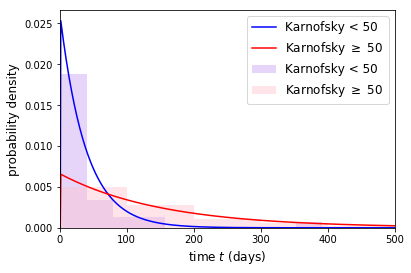
\includegraphics[width=.6\textwidth]{Images/kar/histexp.png} 
\caption{Histogram pro Karnofsky score s vykresleným exponenciálním fitem.}\label{fig:karhist} 
\end{figure}
Na obrázku \ref{fig:karkm} vykreslujeme odhady spolehlivosti a kumulativní intenzity poruch za použití neparametrických modelů. Z obrázku je patrné, že na celém pozorovaném intervalu hodnoty spolehlivosti pro skupinu s vyšším Karnofsky score převyšují spolehlivost pro skupinu pacientů s nižší hodnotou skóre. Podobný trend je patrný i pro kumulativní intenzitu poruch. Z obrázku je navíc patrné, že žádný pacient s $KAR < 50 $ se nedožil 400 dní měření. Výrazné rozdíly pro obě skupiny jsou patrné i z hodnot střední doby života uvedené v tabulce \ref{tab:kar}. Ještě výrazněji jsou poté rozdíly zřejmé na mediánové době života.

Co se parametrických modelů týče, daná rozdělení se podařila namodelovat skrze exponenciální, Birnbaumovo a Weibullovo rozdělení. Co se spolehlivosti $R(t)$ týče, exponenciální a Birnbaumův model vyhodnocují velice podobný průběh jako Kaplan Meierův model. Weibullův model nicméně predikuje hodnoty $R(t)$ pro pacienty s nízkým skóre pozorovatelně blíže k hodnotám druhé skupiny. Tyto rozdíly jsou patrné i v případě průběhu intenzity poruch $r(t)$. Zatímco $r(t)$ pro exponenciální rozdělení nabývá konstantních hodnot, u Birnbaumova rozdělení je patrný výrazný peak. U Weibullova rozdělení intenzita poruch pro skupinu s nízkým skóre poměrně rychle konverguje k intenzitě pro druhou skupinu. Zatímco pro skupinu s $KAR \geq 50$ tak všechny modely predikují podobné spolehlivostní funkce, v případě $KAR < 50$ pak Weibullův model dává pacientům naději na delší dožití.

\begin{figure}[htb!]
\centering
  \begin{subfigure}{.4\linewidth}
    \centering
    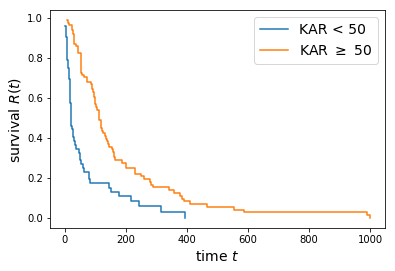
\includegraphics[width=.99\textwidth]{Images/kmkar.png}
  \end{subfigure}%
    \begin{subfigure}{.4\linewidth}
    \centering
    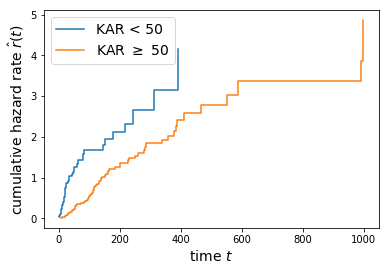
\includegraphics[width=.99\textwidth]{Images/nakar.png}
  \end{subfigure}%     
  \caption{Neparametrické odhady}\label{fig:karkm} 
    \end{figure}
    
      \begin{figure}[htb!]
\centering
    \begin{subfigure}{.4\linewidth}
    \centering
    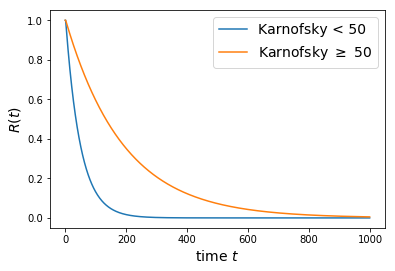
\includegraphics[width=.99\textwidth]{Images/kar/Sexp.png}
  \end{subfigure}%
    \begin{subfigure}{.4\linewidth}
    \centering
    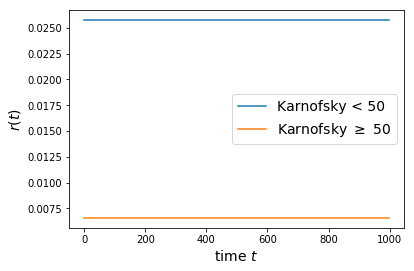
\includegraphics[width=.99\textwidth]{Images/kar/rexp.png}
  \end{subfigure}%
  \caption{Exponential distribution}\label{fig:karexp} 
   \end{figure}   
   
   
 \begin{figure}[htb!]
\centering
    \begin{subfigure}{.4\linewidth}
    \centering
    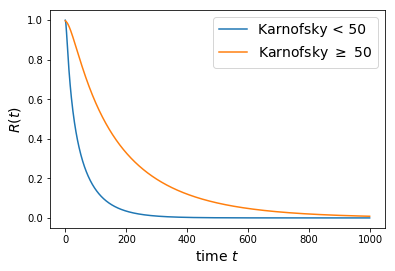
\includegraphics[width=.99\textwidth]{Images/kar/Sbir.png}
  \end{subfigure}%
    \begin{subfigure}{.4\linewidth}
    \centering
    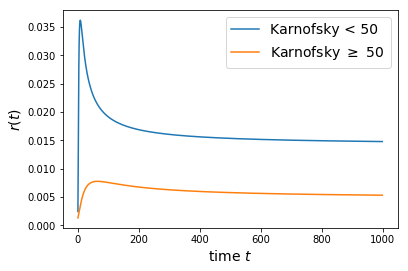
\includegraphics[width=.99\textwidth]{Images/kar/rbir.png}
  \end{subfigure}%
  \caption{Birnbaum distribution}\label{fig:karexp} 
   \end{figure} 
   
   
    \begin{figure}[htb!]
\centering
    \begin{subfigure}{.4\linewidth}
    \centering
    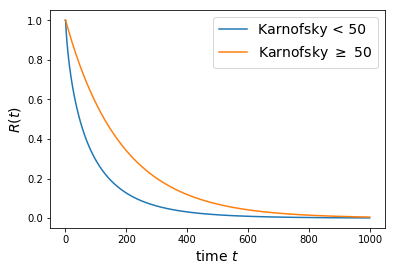
\includegraphics[width=.99\textwidth]{Images/kar/Swei.png}
  \end{subfigure}%
    \begin{subfigure}{.4\linewidth}
    \centering
    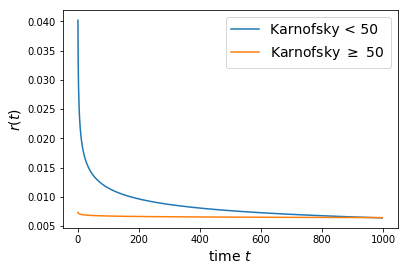
\includegraphics[width=.99\textwidth]{Images/kar/rwei.png}
  \end{subfigure}%
  \caption{Weibull distribution}\label{fig:karexp} 
   \end{figure} 
    
    
\begin{table}[htb!]
\centering
\begin{tabular}{lcccc}
 &  \multicolumn{2}{c}{Karnofsky > 50} & \multicolumn{2}{c}{Karnofsky $\leq$ 50}\\ 
\toprule
Model & mean & median & mean & median \\
\midrule
Kaplan Meier & 159.2 & 112.0 &  57.2 & 21.0\\
Exponential & 153.0 & 106.4 &  39.9 & 27.9 \\
Weibull & 150.0 & 102.9 & 73.1 & 37.8\\
Birnbaum & 153.0 & 100.4 & 40.4 & 22.8\\
\end{tabular}
\caption{Přehled střední a mediánové doby života pro vybrané modely a skupiny.}\label{tab:kar}
\end{table}    
    
\section{Vliv typu rakovinových buněk na čas dožití $T$}
V další části práce se zaměříme na vliv rakovinových buněk na čas přežití $T$. Celkově jsou klasifikovány čtyři typy nádorů, jež jsou společně s průměrnou dobou dožití pro dané skupiny vypsány v tabulce \ref{tab:nadory}. Na první pohled je tedy patrné, že typ nádorů výrazně ovlivňuje dobu přežití pacientů. Na obrázku \ref{fig:cellkm} proto vykreslujeme odhady $R(t)$ pro jednotlivé skupiny nádorů. Z obrázku je zřejmé, že typ adeno je výrazně fatálnější nežli ostatní typy. Proto se zaměříme na porovnání času dožití $T$ pro pacienty s tímto typem nádoru s dobou dožití pro pacienty s jinými typy nádorů.
\begin{table}[htb!]
\centering
\begin{tabular}{lcccc}
    & squamous & smallcell & adeno &  large \\
    \toprule
střední doba života & 200.2 & 71.7 & 64.1 & 166.1
\end{tabular}\caption{Střední doba života pro jednotlivé typy nádorů.}\label{tab:nadory}
\end{table}  
  \begin{figure}[htb!]
\centering
    \begin{subfigure}{.4\linewidth}
    \centering
    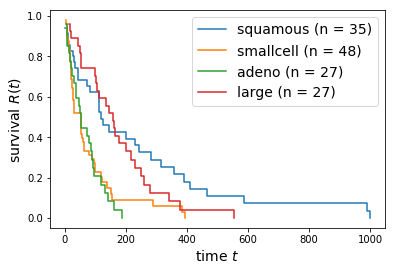
\includegraphics[width=.99\textwidth]{Images/kmcell.png}
  \end{subfigure}%
    \begin{subfigure}{.4\linewidth}
    \centering
    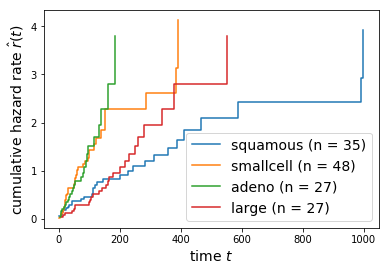
\includegraphics[width=.99\textwidth]{Images/nacell.png}
  \end{subfigure}%\
  \caption{Neparametrické modely}\label{fig:cellkm} 
   \end{figure}
   
     \begin{figure}[htb!]
\centering
    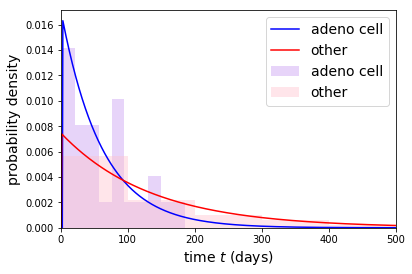
\includegraphics[width=.6\textwidth]{Images/cell/histexp.png}
  \caption{Histogram pro typ buněk s exponenciálním fitem }\label{fig:cellexp} 
   \end{figure} 
   
Na obrázku \ref{fig:adenosdf} vykreslujeme odhady spolehlivostní funkce a kumulativní intenzity poruch pro neparametrické modely. Z obou křivek ja patrný výrazný vliv nádoru typu adeno na dobu přežití. Z parametrických modelů bylo možno použít modely s exponenciálním a Birnbaumovým rozdělením. U intenzity poruch $r(t)$ pro adeno buňky byly u obou modelů pozorovány zhruba dvojnásobné hodnoty oproti intenzitě poruch pro druhou skupinu. 
   
  \begin{figure}[htb!]
\centering
    \begin{subfigure}{.4\linewidth}
    \centering
    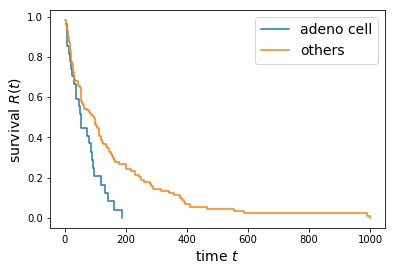
\includegraphics[width=.99\textwidth]{Images/kmadeno.png}
  \end{subfigure}%
    \begin{subfigure}{.4\linewidth}
    \centering
    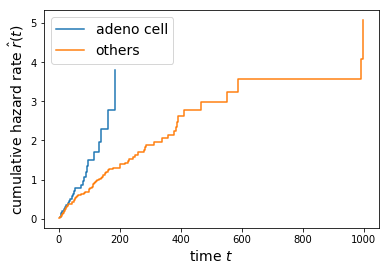
\includegraphics[width=.99\textwidth]{Images/nadeno.png}
  \end{subfigure}%\
  \caption{Neparametrické modely}\label{fig:adenosdf} 
   \end{figure}   
   
   
     \begin{figure}[htb!]
\centering
    \begin{subfigure}{.4\linewidth}
    \centering
    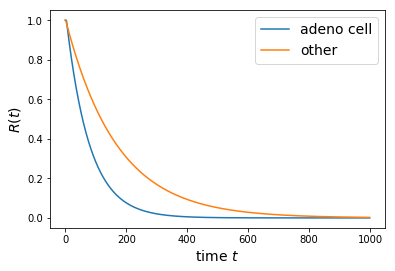
\includegraphics[width=.99\textwidth]{Images/cell/Sexp.png}
  \end{subfigure}%
    \begin{subfigure}{.4\linewidth}
    \centering
    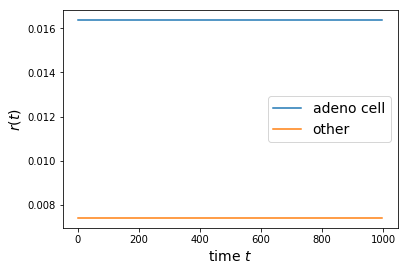
\includegraphics[width=.99\textwidth]{Images/cell/rexp.png}
  \end{subfigure}%
  \caption{Exponential distribution}\label{fig:karexp} 
   \end{figure}   
   
    \begin{figure}[htb!]
\centering
    \begin{subfigure}{.4\linewidth}
    \centering
    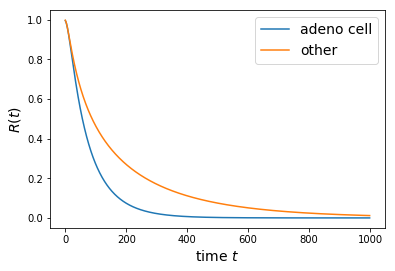
\includegraphics[width=.99\textwidth]{Images/cell/Sbir.png}
  \end{subfigure}%
    \begin{subfigure}{.4\linewidth}
    \centering
    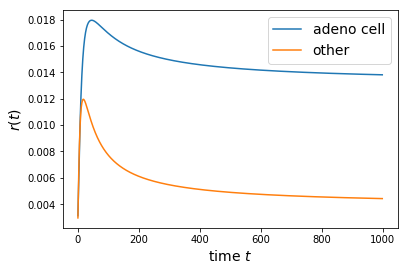
\includegraphics[width=.99\textwidth]{Images/cell/rbir.png}
  \end{subfigure}%
  \caption{Birnbaum distribution}\label{fig:karexp} 
   \end{figure} 

Fatální následky adeno buněk poté potvrzuje přehled středních dob přežití v tabulce \ref{tab:adeno}. Všechny modely se hodnotami téměř shodují na pozorování, že střední doba přežití pro pacienty s nádory typu adeno je cca poloviční oproti všem ostatním typům nádorů dohromady. 

\begin{table}[htb!]
\centering
\begin{tabular}{lcccc}
 &  \multicolumn{2}{c}{adeno} & \multicolumn{2}{c}{other} \\ 
\toprule
Model & mean & median & mean & median \\
\midrule
Kaplan Meier & 59.0 & 51.0 & 142.6 & 95.0 \\
Exponential & 64.1 & 45.4 & 135.5 & 94.4 \\
Birnbaum & 63.8 & 44.9 & 135.0 & 70.4\\
\end{tabular}
\caption{Přehled střední a mediánové doby života pro vybrané modely a skupiny.}\label{tab:adeno}
\end{table}


\section{Vliv věku pacienta na čas dožití $T$}
Dalším faktorem potenciálně ovlivňujícím dobu přežití je věk pacienta. Z tohoto důvodu dělíme pozorované pacienty do skupin s věkem přesahujícím a nepřesahujícím hranici 60 let. Jak ukazuje obrázek \ref{fig:karexasdp}, v rozděleních pro obě skupiny tentokrát není patrný tak výrazný rozdíl jako v předešlých případech.
  \begin{figure}[htb!]
\centering
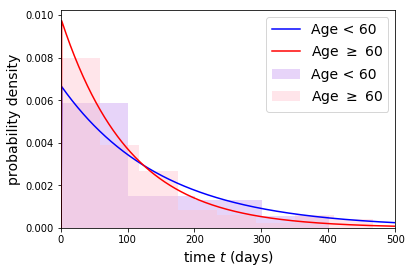
\includegraphics[width=.6\textwidth]{Images/age/histexp.png}
  \caption{Histogram pro vybrané věkové skupiny s exponenciálním fitem.}\label{fig:karexasdp} 
   \end{figure}    
Na obrázku \ref{fig:agxxae} vykreslujeme odhad $R(t)$ pro neparametrický model. Odhadovaná spolehlivostní funkce se pro nízké hodnoty $t$ pro obě skupiny téměř shoduje. Od určitého bodu nicméně ve spolehlivosti získávají výhodu mladší pacienti. 
  \begin{figure}[htb!]
\centering
    \begin{subfigure}{.4\linewidth}
    \centering
    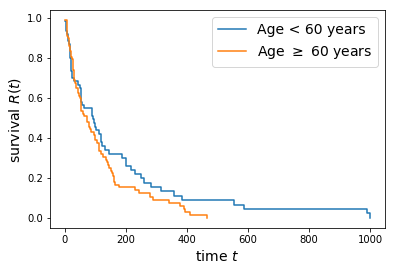
\includegraphics[width=.99\textwidth]{Images/kmage.png}
  \end{subfigure}%
    \begin{subfigure}{.4\linewidth}
    \centering
    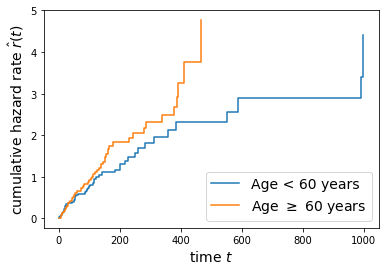
\includegraphics[width=.99\textwidth]{Images/naage.png}
  \end{subfigure}%
  \caption{Neparametrické modely}\label{fig:agxxae} 
   \end{figure}
Podobné výsledky jsou patrné i u parametrických modelů. V tomto případě se kromě exponenciálního rozdělení stává výhodné použít též rozdělení Birnbaumovo či Weibullovo. Na příslušných intenzitách poruch je totiž poměrně zjevné, že v prvních dnech je intenzita poruch pro obě skupiny podobná. Poté se nicméně do výhody dostávají mladší pacienti. To lze interpretovat tak, že pro silně nemocné pacienty umírající v krátkém horizontu po začátku měření nízký věk nijak nedokáže zabránit úmrtí. V delším časovém horizontu se nicméně ukazuje vyšší odolnost mladších pacientů.   
  \begin{figure}[htb!]
\centering
    \begin{subfigure}{.4\linewidth}
    \centering
    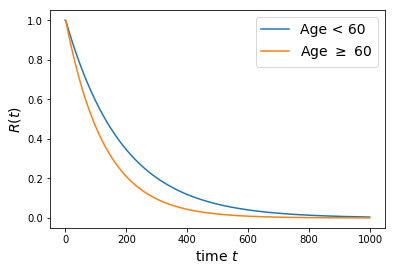
\includegraphics[width=.99\textwidth]{Images/age/Sexp.png}
  \end{subfigure}%
    \begin{subfigure}{.4\linewidth}
    \centering
    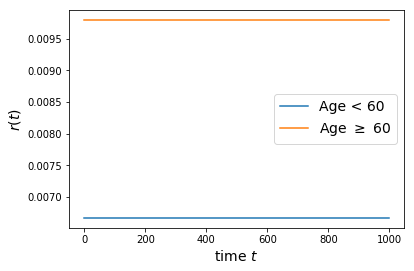
\includegraphics[width=.99\textwidth]{Images/age/rexp.png}
  \end{subfigure}%
  \caption{Exponential distribution}\label{fig:karexp} 
   \end{figure}   
   
    \begin{figure}[htb!]
\centering
    \begin{subfigure}{.4\linewidth}
    \centering
    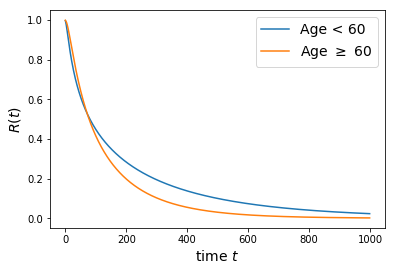
\includegraphics[width=.99\textwidth]{Images/age/Sbir.png}
  \end{subfigure}%
    \begin{subfigure}{.4\linewidth}
    \centering
    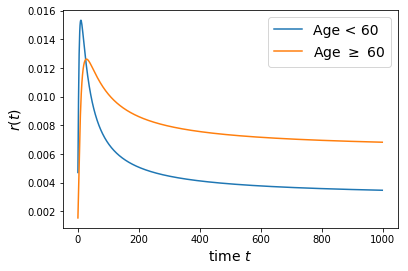
\includegraphics[width=.99\textwidth]{Images/age/rbir.png}
  \end{subfigure}%
  \caption{Birnbaum distribution}\label{fig:karexp} 
   \end{figure} 
   
       \begin{figure}[htb!]
\centering
    \begin{subfigure}{.4\linewidth}
    \centering
    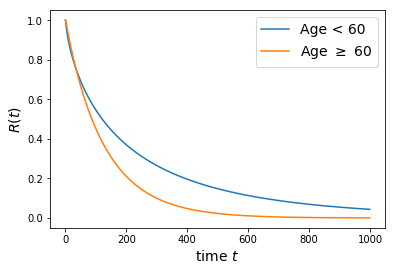
\includegraphics[width=.99\textwidth]{Images/age/Swei.png}
  \end{subfigure}%
    \begin{subfigure}{.4\linewidth}
    \centering
    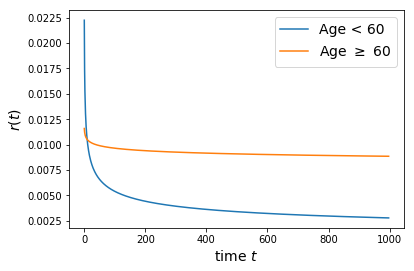
\includegraphics[width=.99\textwidth]{Images/age/rwei.png}
  \end{subfigure}%
  \caption{Weibull distribution}\label{fig:karexp} 
   \end{figure} 
Podíváme-li se na střední doby života pro jednotlivé modely v tabulce \ref{tab:age}, zjišťujeme, že v dlouhodobém horizontu je střední doba přežití mladších pacientů pro všechny modely znatelně vyšší. Velmi výrazné rozdíly jsou poté patrné u modelu s Weibullovým rozdělením, které mladším pacientům přisuzuje výrazně vyšší střední dobu přežití nežli ostatní modely.

\begin{table}[htb!]
\centering
\begin{tabular}{lcccc}
 &  \multicolumn{2}{c}{Age > 60} & \multicolumn{2}{c}{Age $\leq$ 60}\\ 
\toprule
Model & mean & median & mean & median \\ 
\midrule
Kaplan Meier & 104.4 & 72.0 & 155.6 & 92.0 \\
Exponential & 103.1 & 71.8 & 150.1 & 105.0 \\
Birnbaum & 102.5 & 62.5 & 149.6 & 64.6\\
Weibull & 103.3 & 69.8 &201.8 & 97.1 \\
\end{tabular}
\caption{Přehled střední a mediánové doby života pro vybrané modely a skupiny.}\label{tab:age}
\end{table}


\section{Vliv typu léčby na čas dožití $T$}
Posledním zkoumaným faktorem je typ léčby. Zjišťujeme tedy jak se liší doba dožití pro pacienty léčenými standardně oproti testované léčbě. Na základě vykreslených histogramů na obrázku \ref{fig:trcxveat} nicméně na první pohled nejsou patrné výrazné rozdíly.
  \begin{figure}[htb!]
\centering 
    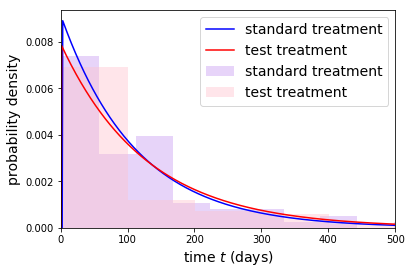
\includegraphics[width=.6\textwidth]{Images/treat/histexp.png}
  \caption{Histogram pro různé typy léčby s exponenciálním fitem.}\label{fig:trcxveat} 
  \end{figure}
Odhad spolehlivostní funkce neparametrického modelu pro dva typy léčby vykreslený na obrázku \ref{fig:tsdfsdfreat} je zajímavý tím, že pro nízké hodnoty $t$ dosahuje lepších výsledků léčba standardní, ale cca od čsu $t = 200$ dnů je nabývá vyšších hodnot spolehlivostní funkce pro placebo. Co se parametrických modelů týče, ačkoliv křivky pro $R(t)$ jsou u obou skupin téměř identické, jsou patrné rozdíly u $r(t)$. V dlouhodobém horizontu je totiž intenzita poruch pro testovanou léčbu pozorovatelně nižší.
  \begin{figure}[htb!]
\centering 
    \begin{subfigure}{.4\linewidth}
    \centering
    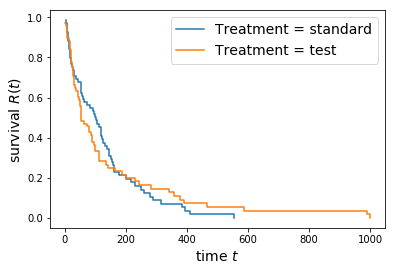
\includegraphics[width=.99\textwidth]{Images/kmtreat.png}
    \label{fig:km1}
  \end{subfigure}%
    \begin{subfigure}{.4\linewidth}
    \centering
    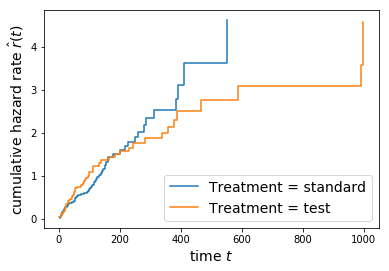
\includegraphics[width=.99\textwidth]{Images/natreat.png}
    \label{fig:km1}
  \end{subfigure}% 
  \caption{Neparametrické modely}\label{fig:tsdfsdfreat} 
  \end{figure}
    \begin{figure}[htb!]
\centering
    \begin{subfigure}{.4\linewidth}
    \centering
    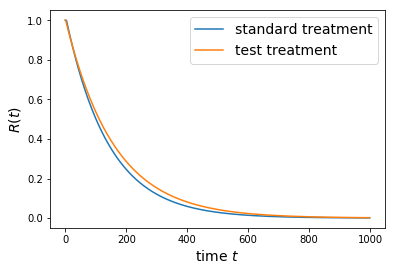
\includegraphics[width=.99\textwidth]{Images/treat/Sexp.png}
  \end{subfigure}%
    \begin{subfigure}{.4\linewidth}
    \centering
    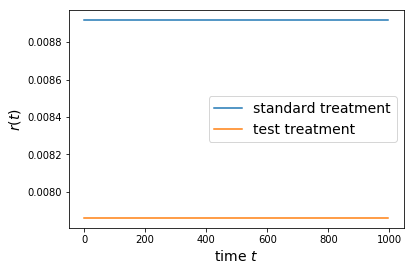
\includegraphics[width=.99\textwidth]{Images/treat/rexp.png}
  \end{subfigure}%
  \caption{Exponential distribution}\label{fig:karexp} 
   \end{figure}   
    \begin{figure}[htb!]
\centering
    \begin{subfigure}{.4\linewidth}
    \centering
    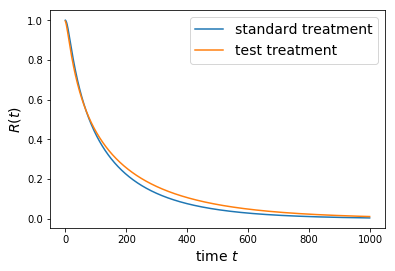
\includegraphics[width=.99\textwidth]{Images/treat/Sbir.png}
  \end{subfigure}%
    \begin{subfigure}{.4\linewidth}
    \centering
    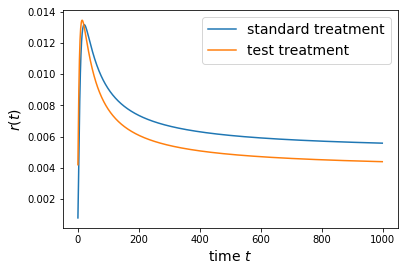
\includegraphics[width=.99\textwidth]{Images/treat/rbir.png}
  \end{subfigure}%
  \caption{Birnbaum distribution}\label{fig:karexp} 
   \end{figure} 
Pozitivní vliv placeba na střední dobu přežití naznačuje i tabulka \ref{tab:treasdat}. U všech modelů se totiž ukázala mírně delší střední doba přežití pro pacienty léčené placebem.   
\begin{table}[htb!]
\centering
\begin{tabular}{lcccc}
 &  \multicolumn{2}{c}{standard} & \multicolumn{2}{c}{test}\\ 
\toprule
Model & mean & median & mean & median \\
\midrule
Kaplan Meier & 116.2 & 103.0 & 132.0 & 53.0 \\
Exponential & 115.2 & 80.8 & 128.2 & 89.2\\
Birnbaum & 113.0  & 63.1 & 129.6 & 64.5 \\
\end{tabular}
\caption{Přehled střední a mediánové doby života pro vybrané modely a skupiny.}\label{tab:treasdat}
\end{table}


  
\newpage


\section{Coxův model}
V rámci předchozí sekce jsme představili sadu modelů predikujících spolehlivost a intenzitu poruch pro vybrané kategorie. Vždy jsme se nicméně omezovali pouze na kategorie jedné proměnné. Jakmile bychom chtěli predikovat dobu dožití pro více zúžený výběr, či dokonce pro jediné pozorování, přestává být tento způsob modelování efektivní. V praxi je tak v takových případech praktičtější použít inovativnější modely. V našem případě modelujeme intenzitu poruch pro vstupní parametry $\textbf{X}$ skrze tzv. Coxův model \cite{cox} ve tvaru
\begin{equation}\label{cox}
r(t\vert \textbf{X}) = r_0(t)\exp(\beta_1X_1 + \dots + \beta_6X_6),
\end{equation}
kde $\beta_1,\dots,\beta_6 \in \mathbb{R} $ jsou koeficienty modelu a $r_0(t)$ značí tzv. baseline hazard. Koeficienty modelu nafitovaného na 137 pozorováních z naší datové množiny jsou uvedeny v tabulce \ref{tab:asdasssd}.
\begin{table}[htb!]
\centering
\begin{tabular}{lc}
proměnná & koeficient \\ 
 \toprule
Age         &   -0.008549 \\
Celltype=large       &   -0.788672 \\
Celltype=smallcell   &   -0.331813 \\
Celltype=squamous    &   -1.188299 \\
Karnofsky score      &   -0.032622 \\
Months from Diagnosis  & -0.000092  \\
Prior therapy=yes    &    0.072327 \\
Treatment=test       &    0.289936 
\end{tabular}
\caption{Koeficienty Coxova modelu.}\label{tab:asdasssd}
\end{table}
Míru kvality klasifikace Coxova modelu měříme v metrice analogické k ploše pod ROC křivkou, v tzv. Harrell's concordance indexu označového též jako c-index \cite{cox}. Ten využijeme k analýze potenciálu jednotlivých proměnných pro odhad intenzity rizika. Coxův model opakovaně natrénujeme pouze pro jednu proměnnou a následně porovnáme c-indexy pro jednotlivé modely. Přehled c-indexů je vypsán v tabulce \ref{tab:asdasd}. Odtud je zřejmé, že čistě na základě Karnofsky score je možno dosáhnout poměrně vysoké hodnoty c-indexu. To ve shodě s našimi poznatky z předchozí sekce ukazuje, že pro analýzu přežití je Karnofsky score nejvýznamnější pozorovanou veličinou. 

\begin{table}[htb!]
\centering
\begin{tabular}{lc}
proměnná & c-index \\ 
 \toprule
Karnofsky score       &   0.709280 \\
Celltype=smallcell    &   0.572581 \\
Celltype=large        &   0.561620 \\
Celltype=squamous     &   0.550545 \\
Treatment=test        &   0.525386 \\
Age          &   0.515107 \\
Months from Diagnosis &   0.509030 \\
Prior therapy=yes     &   0.494434 
\end{tabular}
\caption{Přehled c-indexů pro Coxovy modely fitované s příslušnou proměnnou.}\label{tab:asdasd}
\end{table}


\section{Závěr}

V rámci této práce jsme se věnovali testování vhodných spolehlivostních modelů pro časy dožití $T$ jednotlivých podskupin z pozorování 137 pacientů. Celkově jsme testovali neparametrické a parametrické modely pro skupiny s různými Karnofsky score, typy nádorů, věkem a typy léčby. Pro odhad spolehlivostní funkce a intenzity poruch se osvědčil Kaplan Meierův a Nelson Aalenův neparametrický model. Z parametrických modelů se i přes širokou škálu testovaných distribucí nejvíce osvědčily modely s exponenciálním a Birnbaumovým rozdělením. Co se jednotlivých skupin týče, pozorovaly jsme výrazné rozdíly pro podskupiny s různým Karnofsky score a typy nádoru. Pro věk pacienta a typ léčby jsme tak jednoznačné rozdíly nepozorovali. Na závěr jsme zkonstruovali Coxův model predikující intenzitu poruch na základě vstupních parametrů. Na základě c-indexu jsme poté pozorovali vliv jednotlivých proměnných, a potvrdili jsme význam Karnofsky score pro výslednou predikci.  





\begin{thebibliography}{9}
\bibitem{cox}\textsc{Fox}, J. Cox Proportional-Hazards Regression for Survival Data, \emph{Appendix to An R and S-PLUS Companion to Applied Regression}, 15 June 2008. \url{https://socialsciences.mcmaster.ca/jfox/Books/Companion-1E/appendix-cox-regression.pdf}

\end{thebibliography}
\end{document}